\setcounter{equation}{0}
\chapter{Model}
\label{chap:model}

LAEs, although not very known, are still galaxies. They are a collection of bodies and matter interacting one with another. This causes particular movements as a whole that should always be present and considered. Two of these main movements are the rotation and expansion. \\

All bodies in the universe feel a gravitational attraction between them. A galaxy starts forming when some of them start to collapse around their center of mass. However, the matter in the universe is not uniformly distributed. There are some lumps of different masses and at distinct distances around the galaxy. This causes its different parts to be pulled more strongly in some directions. As probably the torques don't balance the galaxy starts to spin in a certain way and with a rotational velocity \vrot. \\

If one considers the rotational velocity of a galaxy plus its gravitational collapsing towards its center of mass, an interesting effect is observed. The initial sphere starts to flatten into a disk, just as our Milky Way \footnote{This is the same effect that causes a ball of mass to become a flat pizza when the chef throws it in the air spinning}. However, a very long time has to pass until this takes place. And in LAEs, because they are very young, the material collapsing is still pseudo uniformly distributed in a spherical shape. \\

On another scale, the stars inside this new forming galaxy follow a different time scale. Their duration is much shorter so many supernovas happen during the galaxy's life time. These supreme explosions eject material in all directions. They travel through the body in such a strong way, they can even escape from it. These are called outflows and induce a radial velocity to the galaxy \vout. \\ 

These 3 considerations leave the idea of a model of LAE, that although simple, considers the main galaxy's dynamics. All of them have been previously proposed by different author, but never combined together. This new model consists of the mixture of them.\\

\begin{figure}[h!]
	\begin{center}
		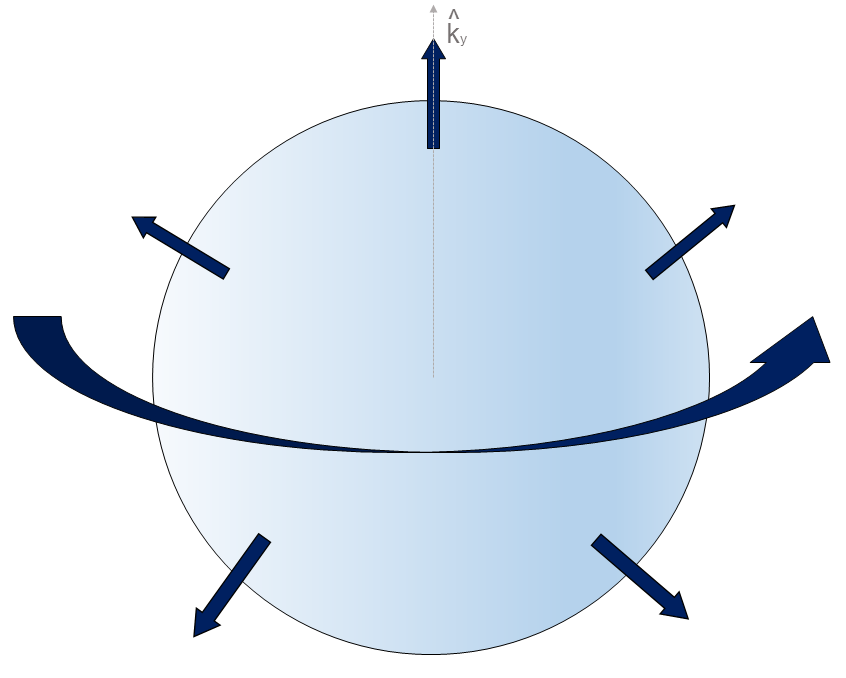
\includegraphics[width=0.6\textwidth]{./figures/chapter2/model}
	\end{center}
	\caption{\textbf{Model:} Spherical LAE with tangential and radial velocity due to rotation and outflows, respectively.
		\label{fig:model}}
\end{figure}

I propose a spherical galaxy composed by H atoms that undergo a solid-body rotation and a radial expansion due to outflows, as seen in Fig. \ref{fig:model}. In this model the velocity of each H atom is described by components in Eqs. \ref{eq:vx} \ref{eq:vy} \ref{eq:vz}. In these, $R$ is the radius of the sphere; $x$, $y$ and $z$ are the position of the atom; and the $\mp$ signs in $v_x$ and $v_y$, respectively, indicate the direction of rotation. This rotation direction goes according to the right hand rule applied to the  $\hat{k}$ unit vector \\

\begin{equation}
v_{x}=\frac{x}{R}v_{\rm out}-\frac{y}{R}v_{\rm rot} 
\label{eq:vx}
\end{equation}

\begin{equation}
v_{y}=\frac{y}{R}v_{\rm out}+\frac{x}{R}v_{\rm rot} 
\label{eq:vy}
\end{equation}

\begin{equation}
v_{z}=\frac{z}{R}v_{\rm out}
\label{eq:vz}
\end{equation}

Apart from these velocities, another key factor needs to be taken into account. This is the mass of the LAE, or in another words, its number of H atoms. For this reason another dimensionless variable is defined, called the optical depth \tauh. \tauh measures the number of H atoms found if one traces a line from the center of the galaxy, to its edge.\\

Now the 3 main model parameters are defined: \vrot, \vout and \tauh. \\


\section{Photon's Path}
In several problems in science it is sometimes really useful to define dimensionless variables of equations. This new formulation has many advantages. For example, now regardless of units, there is always a definition of small. This tends to make the results' analysis much more easier. For this reason, I define a new dimensionless variable $x$ in the model to describe a photon's wavelength.\\

\begin{equation}
\label{eq:x_freq}
x \equiv \frac{(\nu -\nu_{\rm \alpha})}{\Delta\nu_{\rm D}}
\end{equation} 

A photon's wavelength can be also expressed as its reciprocal form of frequency $\nu$. This is defined as $\nu = c/\lambda$, where $c$ is the speed of light and $\lambda$ is the wavelength. So, in Eq. \ref{eq:x_freq}, $\nu$ refers to the photon's frequency and $\nu_{\rm \alpha} = 2.46\times 10^{15}$ Hz is the \lya natural frequency. The denominator $\Delta\nu_{\rm D}$ is defined in Eq. \ref{eq:delta_nuD}.

\begin{equation}
\label{eq:delta_nuD}
\Delta\nu_{\rm D} \equiv \nu_{\rm \alpha}\sqrt{\frac{2kT}{m_pc^2}} \equiv \nu_{\rm \alpha} \frac{v_{\rm th}}{c}
\end{equation} 

$\Delta\nu_{\rm D}$ is the Doppler broadening of the \lya line. It depends on the neutral gas temperature $T$ or equivalently the thermal velocity $v_{\rm th}$ of the atoms. In the model the temperature is $T=10^4$K and the thermal velocity is $v_{\rm th}=12.8$\kms. \\

This variable $x$ is now the parameter that defines how the final wavelength of a photon ends up. If $x < 0$, the final frequency $\nu < \nu_{\rm \alpha}$. This translates to the final wavelength being larger than the \lya natural one. The phenomenon is called a redshift in frequency. If, on the contrary, $x > 0$, the photon suffers a blueshift in frequency. \\

As mentioned before, this is a radiative transfer model. This means that it is necessary to define the way the energy is transfered through the galaxy. For simplicity of the code, the initial emission of photons is taken at the center of the sphere. From here, $100000$ photons are emitted with the natural \lya wavelength. Then, they start to behave as previously described (See Fig. \ref{fig:radiative_transfer}). When each photon is re-emitted, its new wavelength depends merely on the H atom velocity. However its new direction of propagation is random. \\ 

The individual scattering of all the photons is tracked through the complete 3D Hydrogen distribution. Once each photon escapes the galaxy, its final values are stored: position $\vec{r}$, direction of propagation $\hat{k}$, dimensionless frequency $x$, and number of scatterings $N$. When the last photon leaves the galaxy, a histogram of final $x$ values is created. This plot represents the \lya line of the galaxy spectrum.\\


\section{Galaxy's Viewing Angle}
Is important to note that if we stand next to the galaxy, not all of the photons emitted are going to be observed because some will have directions that could never reach our position. For this reason, it is very important to define viewing angle so that only photons that escape within that range are counted in the spectrum. As seen in Fig. \ref{fig:viewing_angle_sketch}, only the photons with escaping direction angle $\theta$ respect to the rotation axis that belongs to the range $[\theta_{min}-\theta_{max}]$ reach the observer. \\

\begin{figure}[h!]
	\begin{center}
		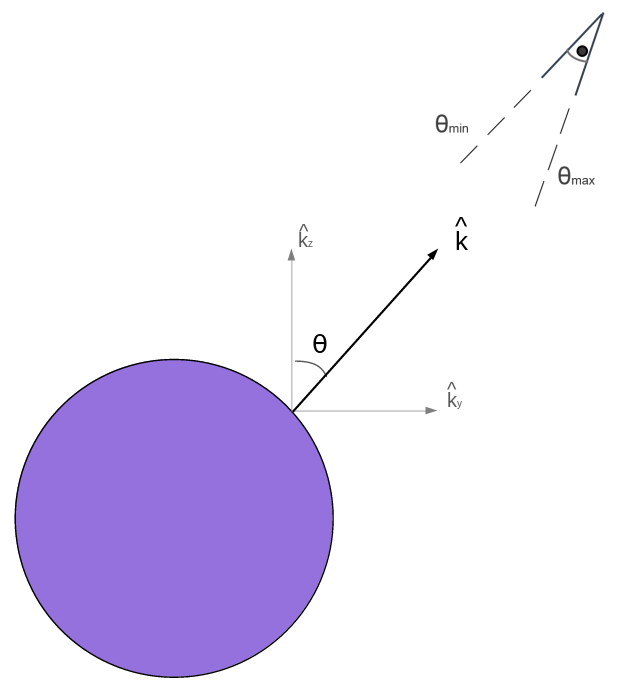
\includegraphics[width=1\textwidth]{./figures/chapter2/viewing_angle_sketch}
	\end{center}
	\caption{\textbf{Viewing Angle Sketch:} The galaxy is in the $y-z$ plane perspective and the eye is located at an specific viewing angle of the sphere. Only photons with a direction that enters in his range of vision can enter to the result.
		\label{fig:viewing_angle_sketch}}
\end{figure}

This consideration creates 2 new parameters, the azimuthal angle and the polar angle. However, the galaxy's movement is symmetrical respect to its rotation axis. This implies that the resulting spectrum will not vary depending on the azimuthal angle. This makes all of the photons with azimuthal viewing angle from $0$ to $2\pi$ have the same result, disregarding the selected polar range. I will choose all of them for statistical reasons. Regarding the polar angle, I will take spectra from 9 different ranges from $0$ to $\pi$ that are uniform in $\cos(\theta)$ and analyze the influence of this effect as well. \\ 

All of the resulting spectra considering the 3 galaxy parameters and the viewing angle are available in the next chapter. 
